\begin{frame}{こんなん出ましたけど??}
   \begin{columns}[t]
    \begin{column}{0.6\textwidth}
      <こんなん出ましたけど??>
      \begin{itemize}
        \item[(1)]<1-> JOBの設定は省略
        \item[(2)]<2-> 結果の表示 \\
		       まだらにならず、きれいな層状に表示\\
		       それっぽくは見えるが??\\
		       ここから詳しくチェック
      \end{itemize}
    \end{column}
    \begin{column}{0.4\textwidth}
      \vspace{-7mm}
      \begin{figure}[htbp]
        \begin{center}
          \begin{overlayarea}{7cm}{15cm}
            \only<2->{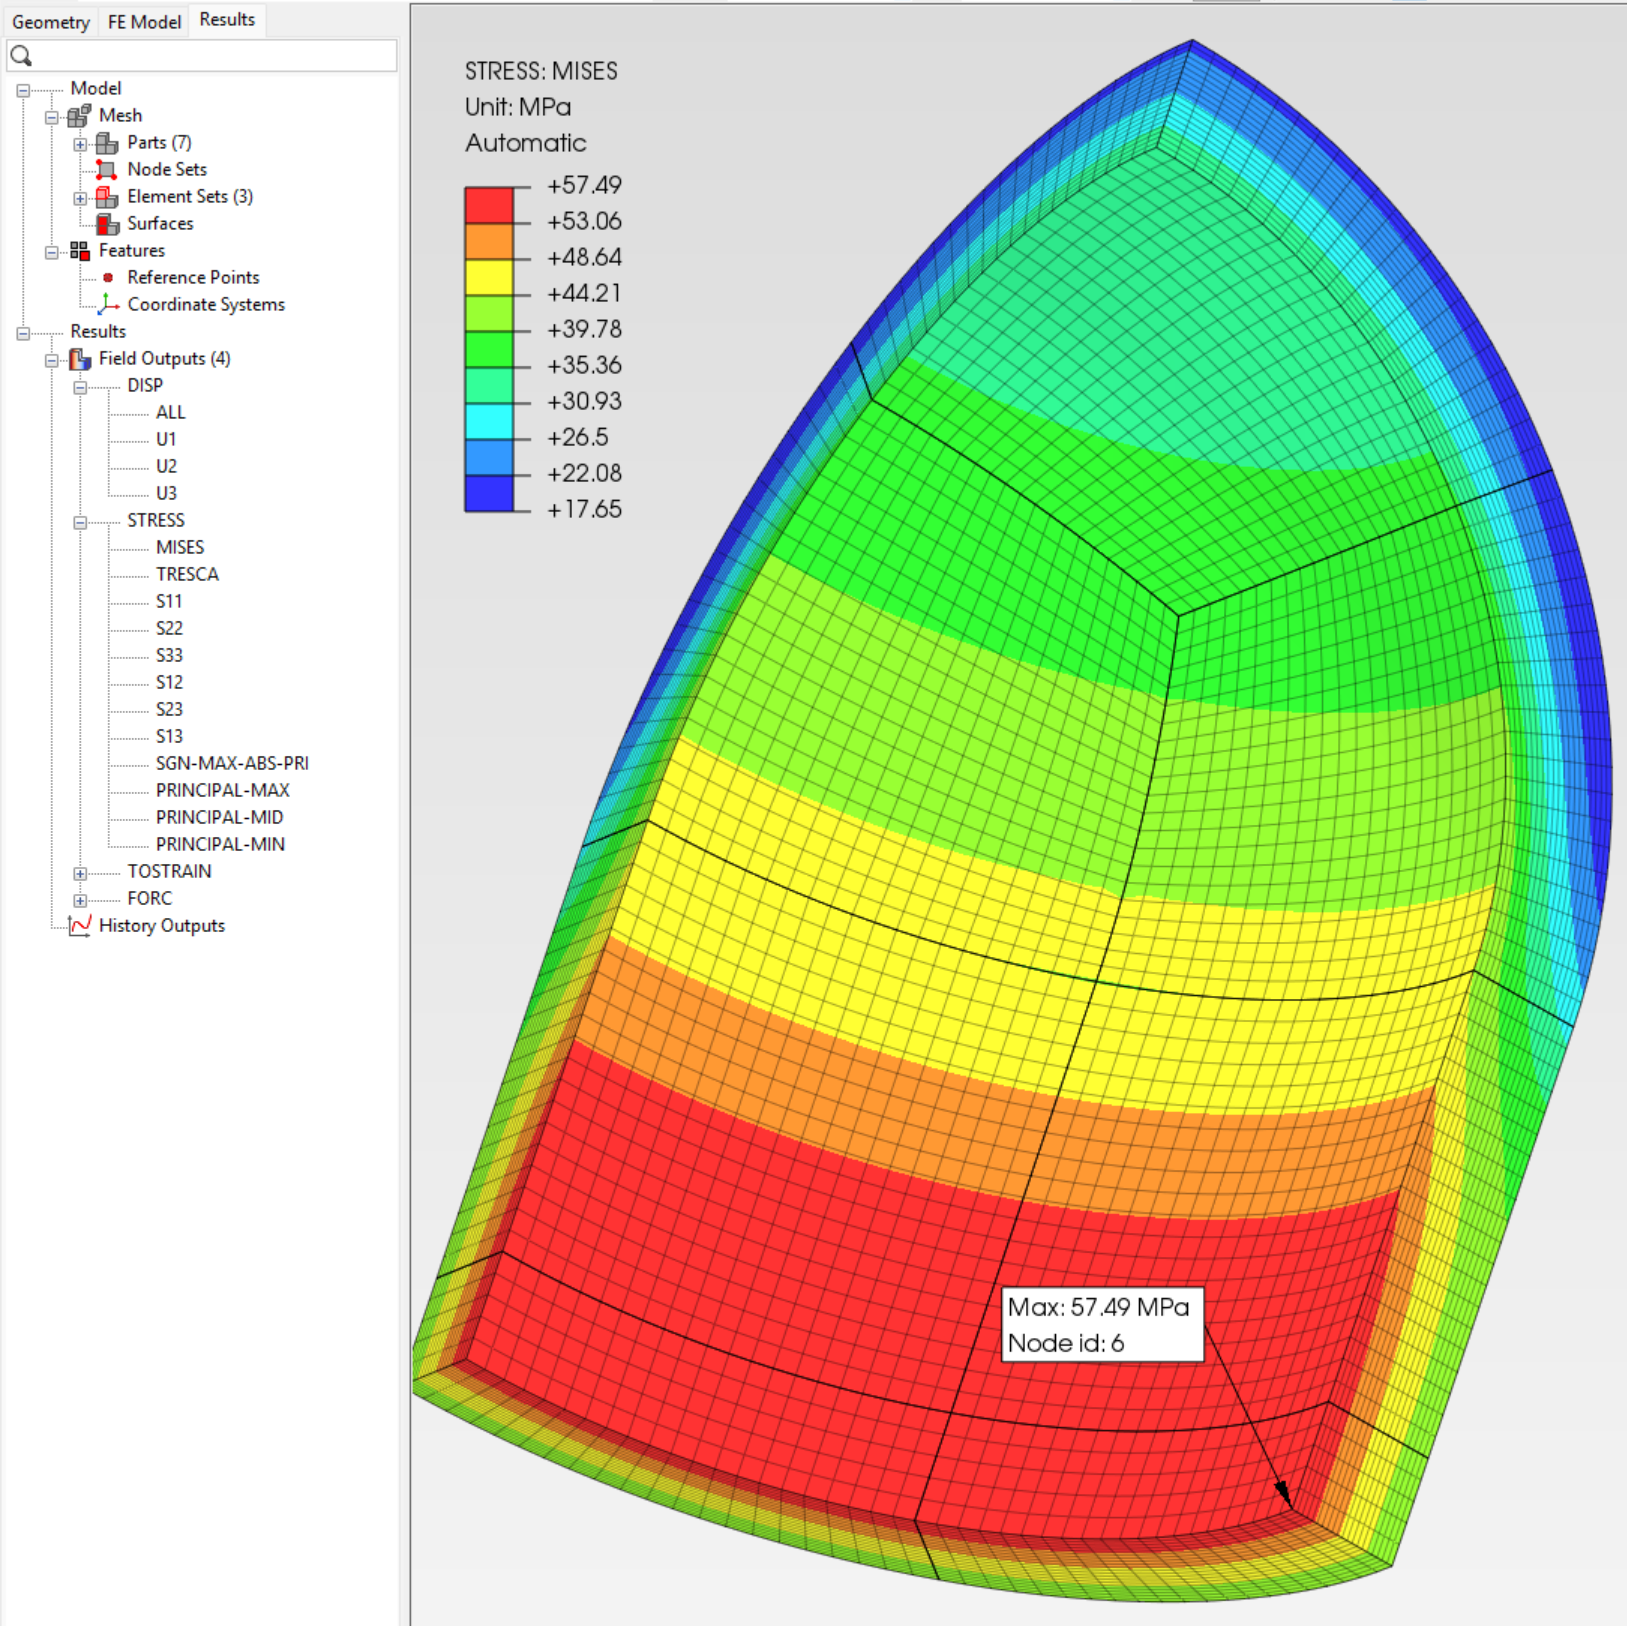
\includegraphics[keepaspectratio,scale=0.30]{images/sc16.png}}
            \caption{ミーゼス応力コンター図}
          \end{overlayarea}
        \end{center}
      \end{figure}
    \end{column}
  \end{columns}
  \only<2>{
    \begin{textblock*}{160pt}(200pt,90pt)
      \begin{tikzpicture}
         \node[rectangle,fill=cud_yellow,text width=90pt,text centered,rounded corners,minimum height=20pt](s) at (1cm,1cm) { \scriptsize ミーゼス応力};
         \draw[->, draw=cud_red, line width=1pt] (10pt,38pt) -- (42pt,110pt);
      \end{tikzpicture}
    \end{textblock*}
  }
\end{frame}
